
\documentclass[10pt]{article}
\usepackage[utf8]{inputenc}
\usepackage{graphicx}
\usepackage{amsmath, amssymb}
\usepackage{geometry}
\usepackage{caption} 
\geometry{a4paper, margin=0.5in, landscape} 

\begin{document}

\section*{Comparative EIS Kinetics Report}
\textbf{Model Structure:} \texttt{R0-p(R1-p(R2,CPE2),CPE1)} \\
\textbf{Used data:} altered data, first 4 points removed and points with $freq > 2e+04$ removed

\begin{center}
    
\includegraphics[width=0.45\textwidth]{../../../../2RC.png}
\end{center}

\renewcommand{\arraystretch}{1.6} 
\begin{table}[h!]
    \centering
    \footnotesize
    \begin{tabular}{|l|c|c|c|c|c|c|}
        \hline
        \textbf{Element} & \textbf{Unit} & \textbf{Bounds} & \textbf{Cauvel\_4\_NaVO3\_24H} & \textbf{Cauvel\_4\_NaVO3\_48H} & \textbf{Cauvel\_4\_NaVO3\_72H} & \textbf{Cauvel\_4\_NaVO3\_168H} \\ \hline
        $R_{0}$ & $\Omega$ & $[1.0e-03, 1.0e+03]$ & $6.49e+01 \pm 4.0e-01$ & $1.84e+01 \pm 2.8e+01$ & $6.60e+01 \pm 1.4e-01$ & $6.92e+01 \pm 2.6e-01$ \\ \hline
        $R_{1}$ & $\Omega$ & $[1.0e+00, 1.0e+08]$ & $2.22e+02 \pm 1.1e+02$ & $5.24e+01 \pm 2.8e+01$ & $3.24e+05 \pm 3.7e+03$ & $2.63e+05 \pm 1.6e+04$ \\ \hline
        $R_{2}$ & $\Omega$ & $[1.0e+00, 1.0e+08]$ & $3.16e+05 \pm 2.2e+03$ & $3.37e+05 \pm 7.0e+03$ & $1.00e+08 \pm 1.0e-04$ & $2.55e+06 \pm 1.4e+01$ \\ \hline
        $Q_{2}$ & $\Omega$$^{-1}$ sec$^{a}$ & $[1.0e-11, 1.0e-03]$ & $5.87e-07 \pm 2.8e-07$ & $9.93e-06 \pm 3.5e-07$ & $1.69e-04 \pm 2.8e-05$ & $2.42e-05 \pm 6.5e-06$ \\ \hline
        $n_{2}$ & - & $[5.0e-01, 1.0e+00]$ & $9.54e-01 \pm 3.2e-02$ & $8.49e-01 \pm 3.2e-03$ & $1.00e+00 \pm 8.6e-02$ & $5.00e-01 \pm 8.1e-02$ \\ \hline
        $Q_{1}$ & $\Omega$$^{-1}$ sec$^{a}$ & $[1.0e-11, 1.0e-03]$ & $9.92e-06 \pm 2.9e-07$ & $1.31e-06 \pm 3.2e-07$ & $1.07e-05 \pm 2.4e-08$ & $1.09e-05 \pm 5.5e-08$ \\ \hline
        $n_{1}$ & - & $[5.0e-01, 1.0e+00]$ & $8.39e-01 \pm 1.9e-03$ & $5.61e-01 \pm 7.7e-02$ & $8.38e-01 \pm 4.4e-04$ & $8.29e-01 \pm 9.2e-04$ \\ \hline
        \textbf{$\chi^2$} & - & -  & $9.686e-05$ & $9.895e-05$ & $4.918e-05$ & $1.318e-04$ \\ \hline

    \end{tabular}
\end{table}


\newpage
\section*{Analysis Results: 24H}
\begin{center}
    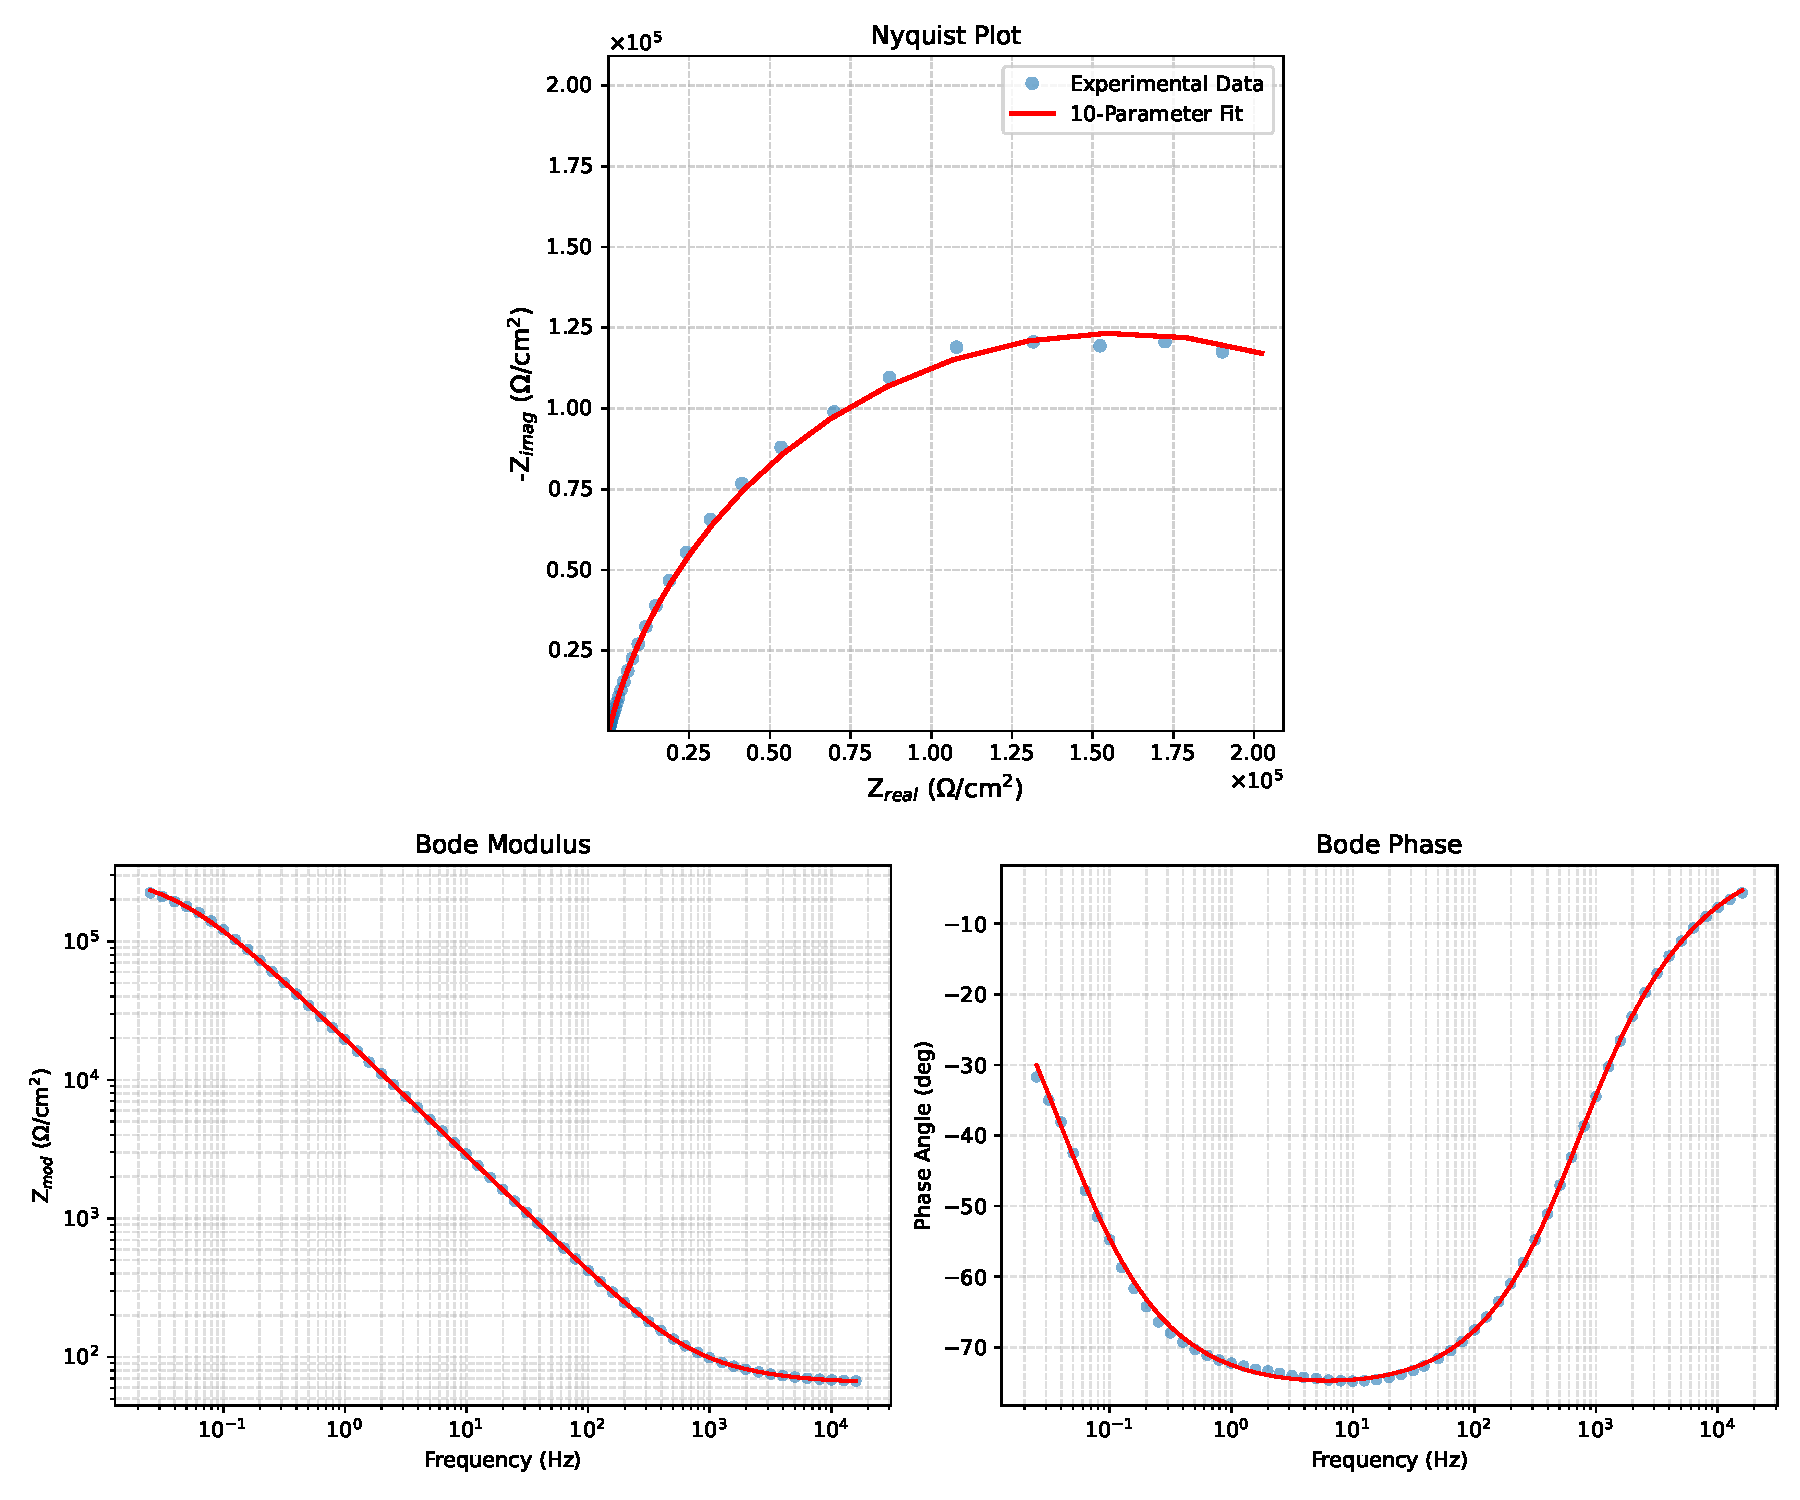
\includegraphics[width=0.7\textwidth]{plots_Cauvel_4_NaVO3_24H_2RC.pdf}
    \captionof{figure}{EIS Fit Results for Cauvel\_4\_NaVO3\_24H}
\end{center}

\newpage
\section*{Analysis Results: 48H}
\begin{center}
    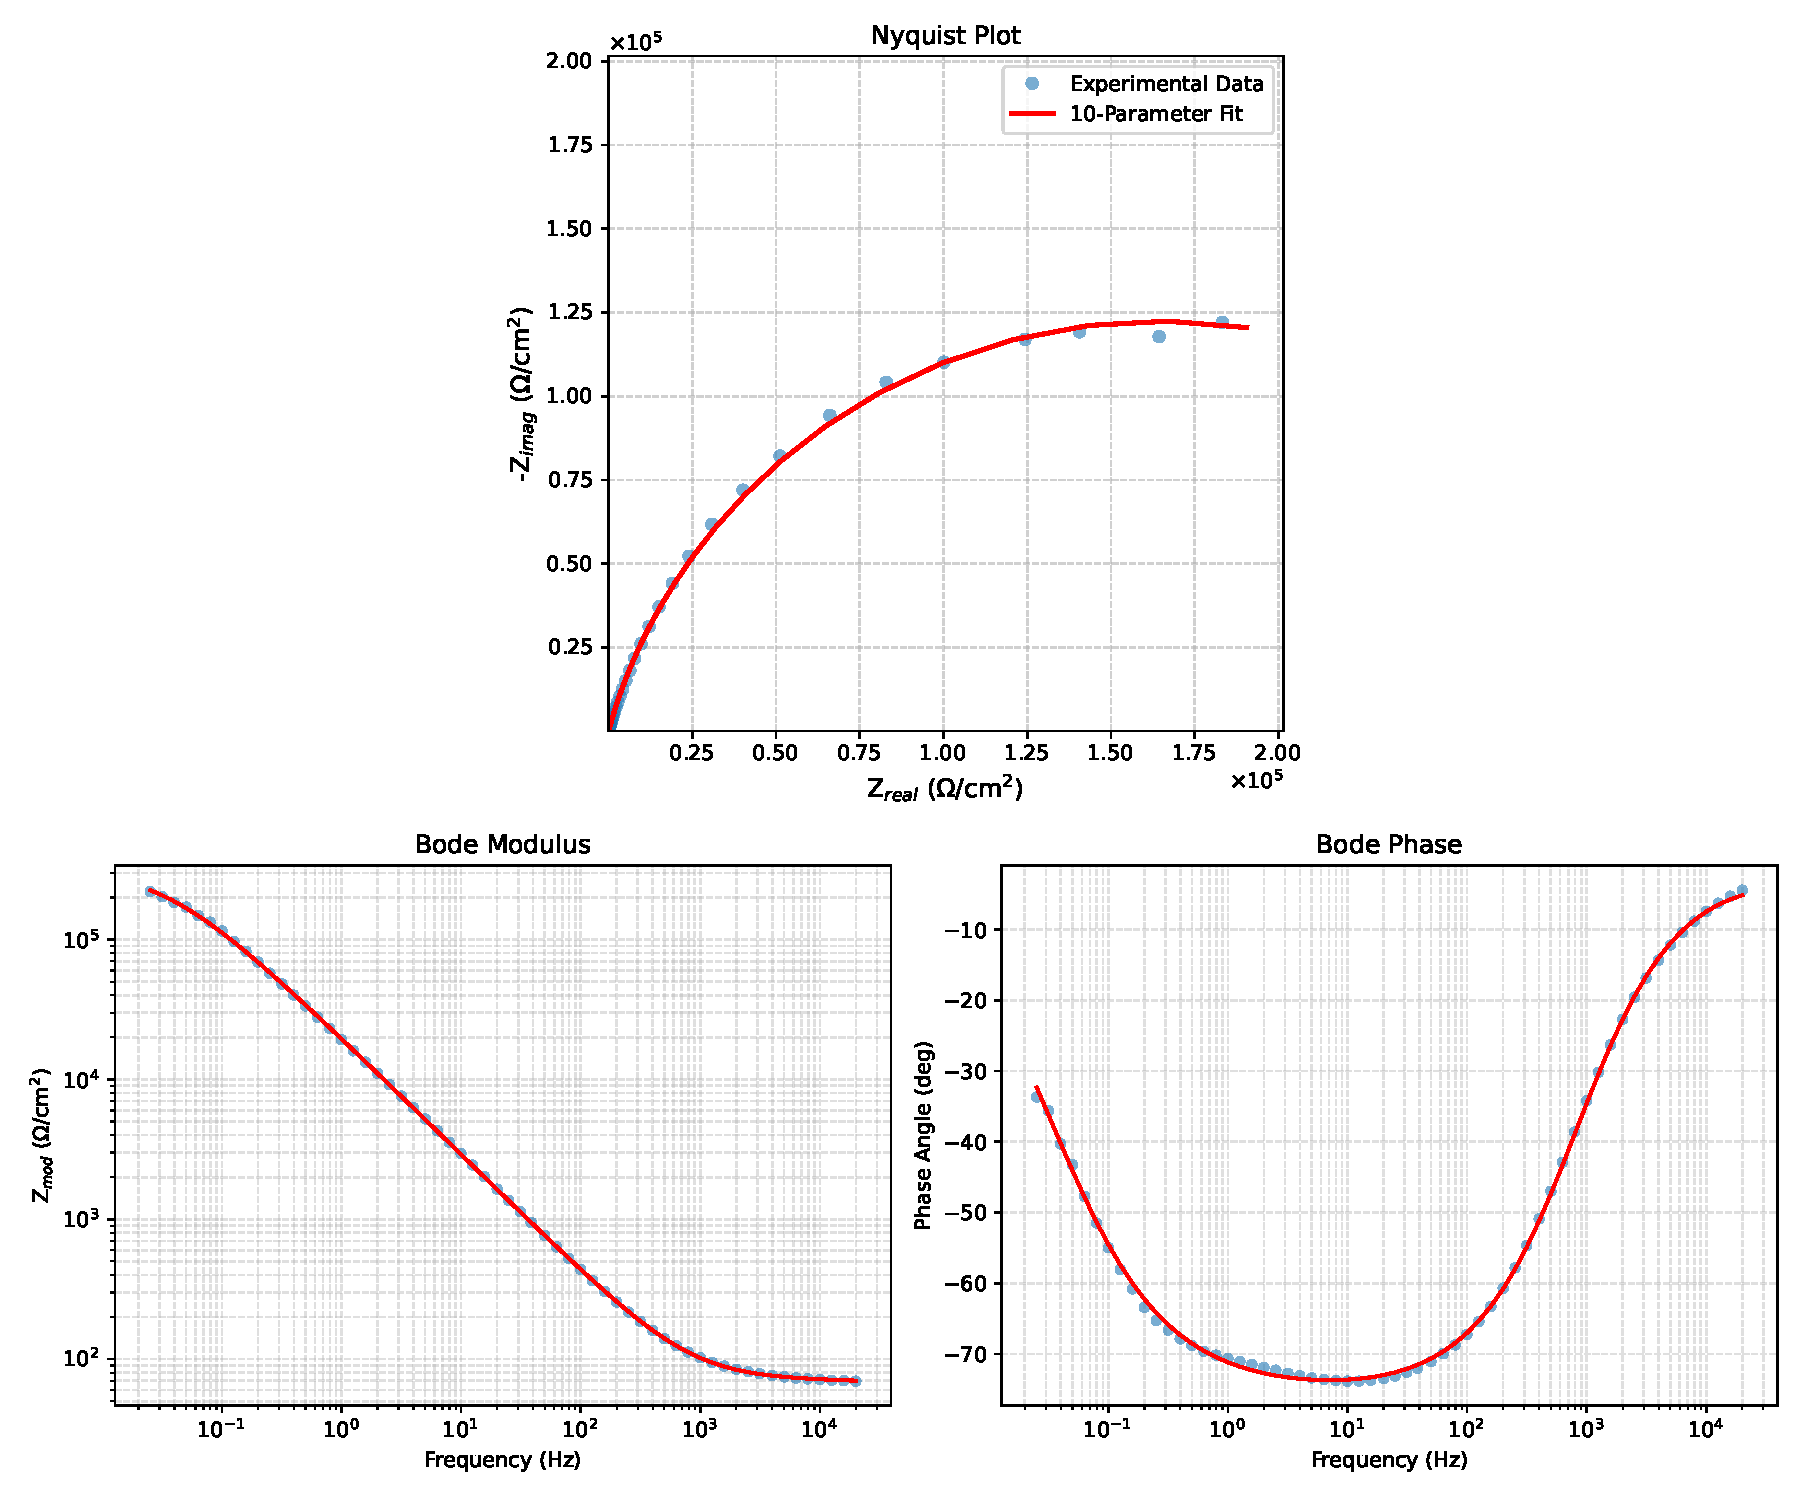
\includegraphics[width=0.7\textwidth]{plots_Cauvel_4_NaVO3_48H_2RC.pdf}
    \captionof{figure}{EIS Fit Results for Cauvel\_4\_NaVO3\_48H}
\end{center}

\newpage
\section*{Analysis Results: 72H}
\begin{center}
    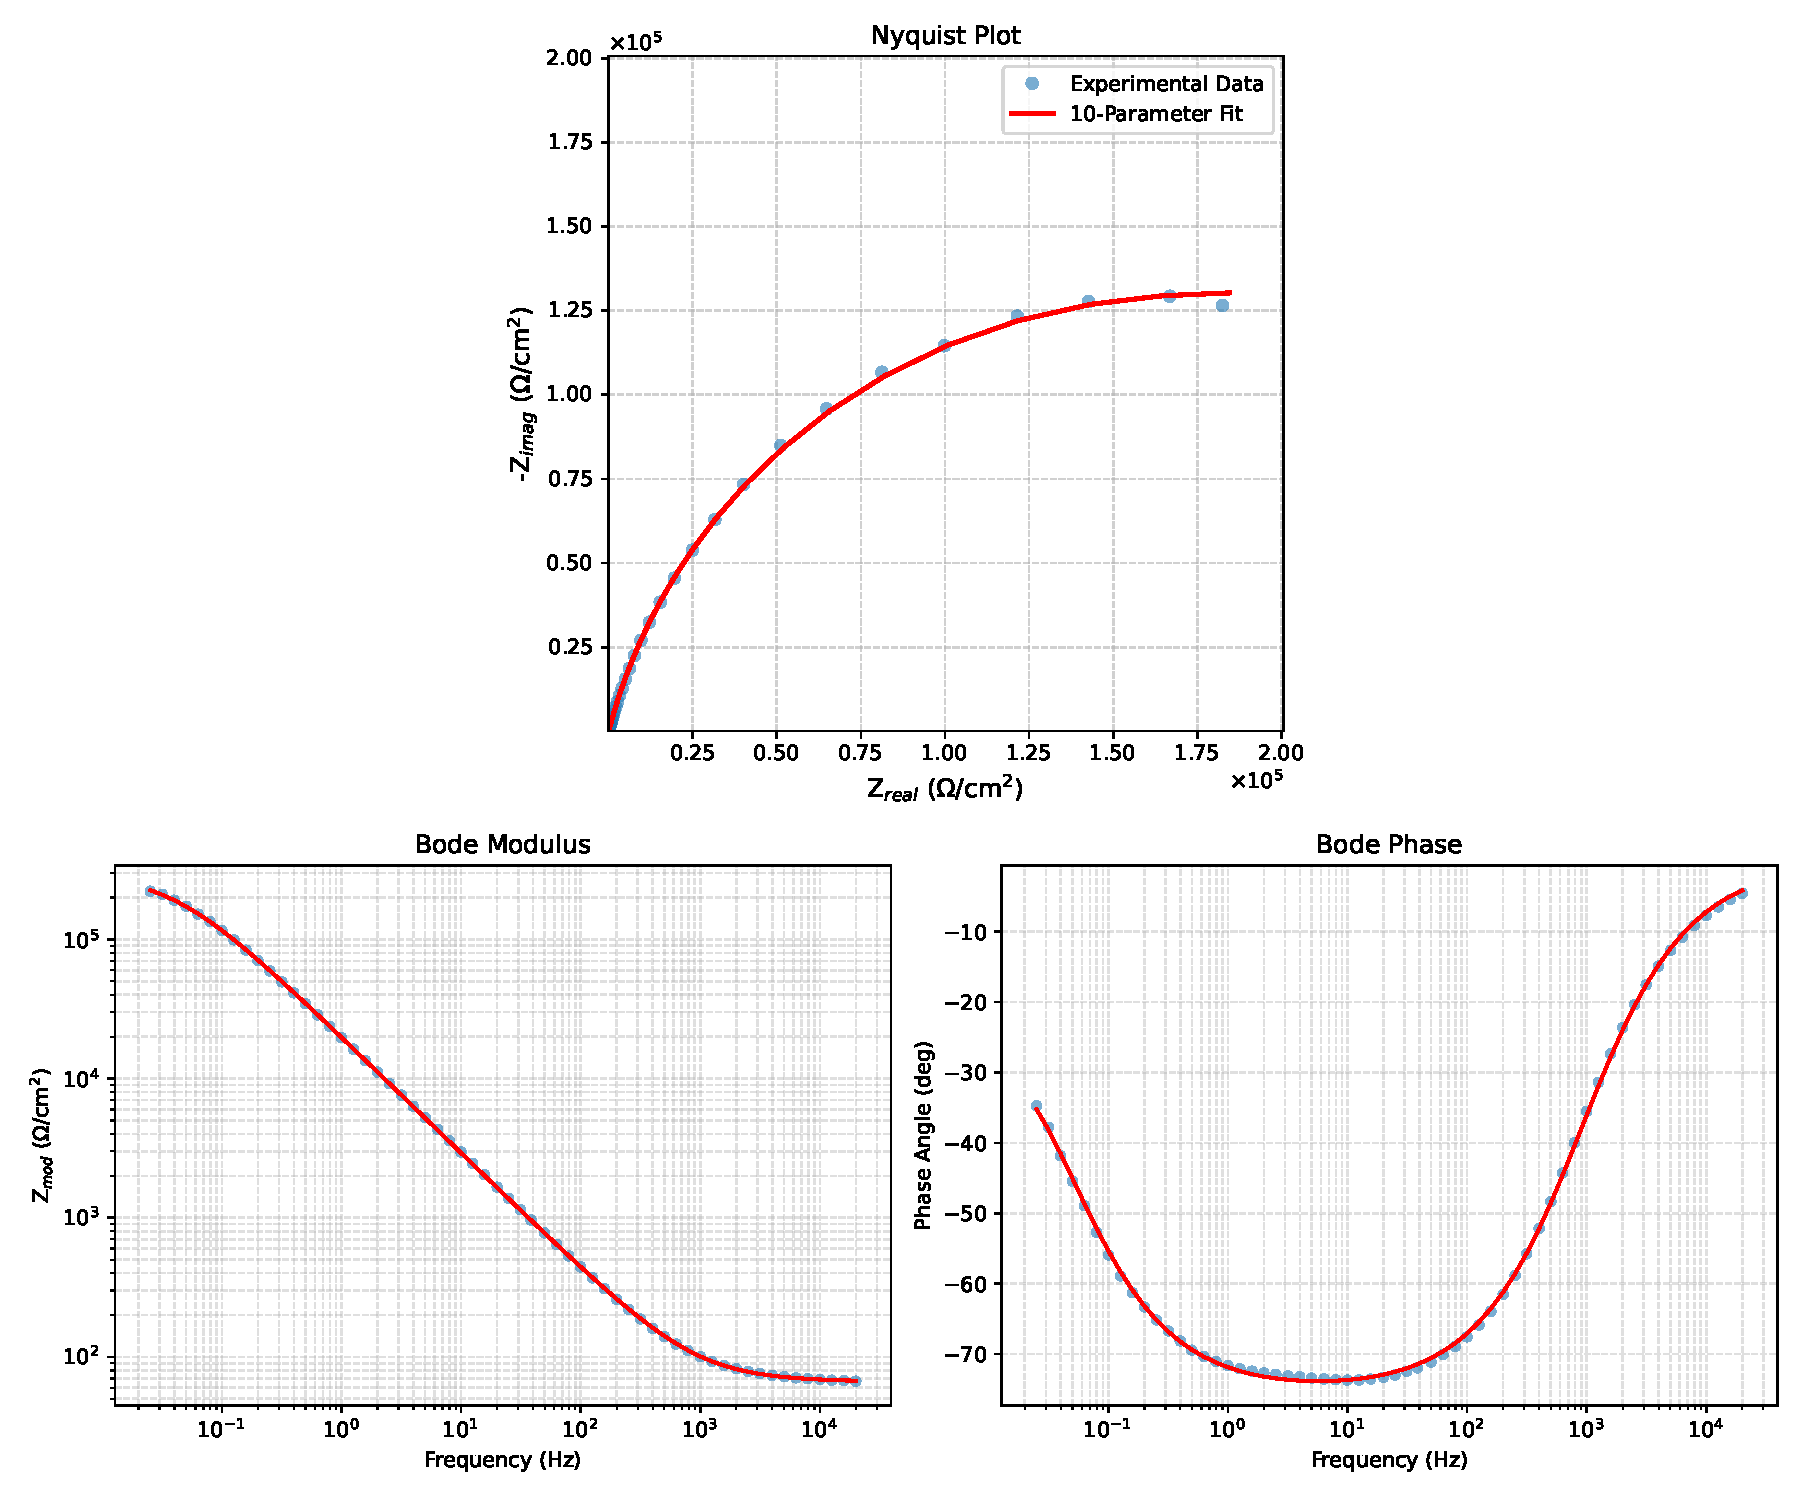
\includegraphics[width=0.7\textwidth]{plots_Cauvel_4_NaVO3_72H_2RC.pdf}
    \captionof{figure}{EIS Fit Results for Cauvel\_4\_NaVO3\_72H}
\end{center}

\newpage
\section*{Analysis Results: 168H}
\begin{center}
    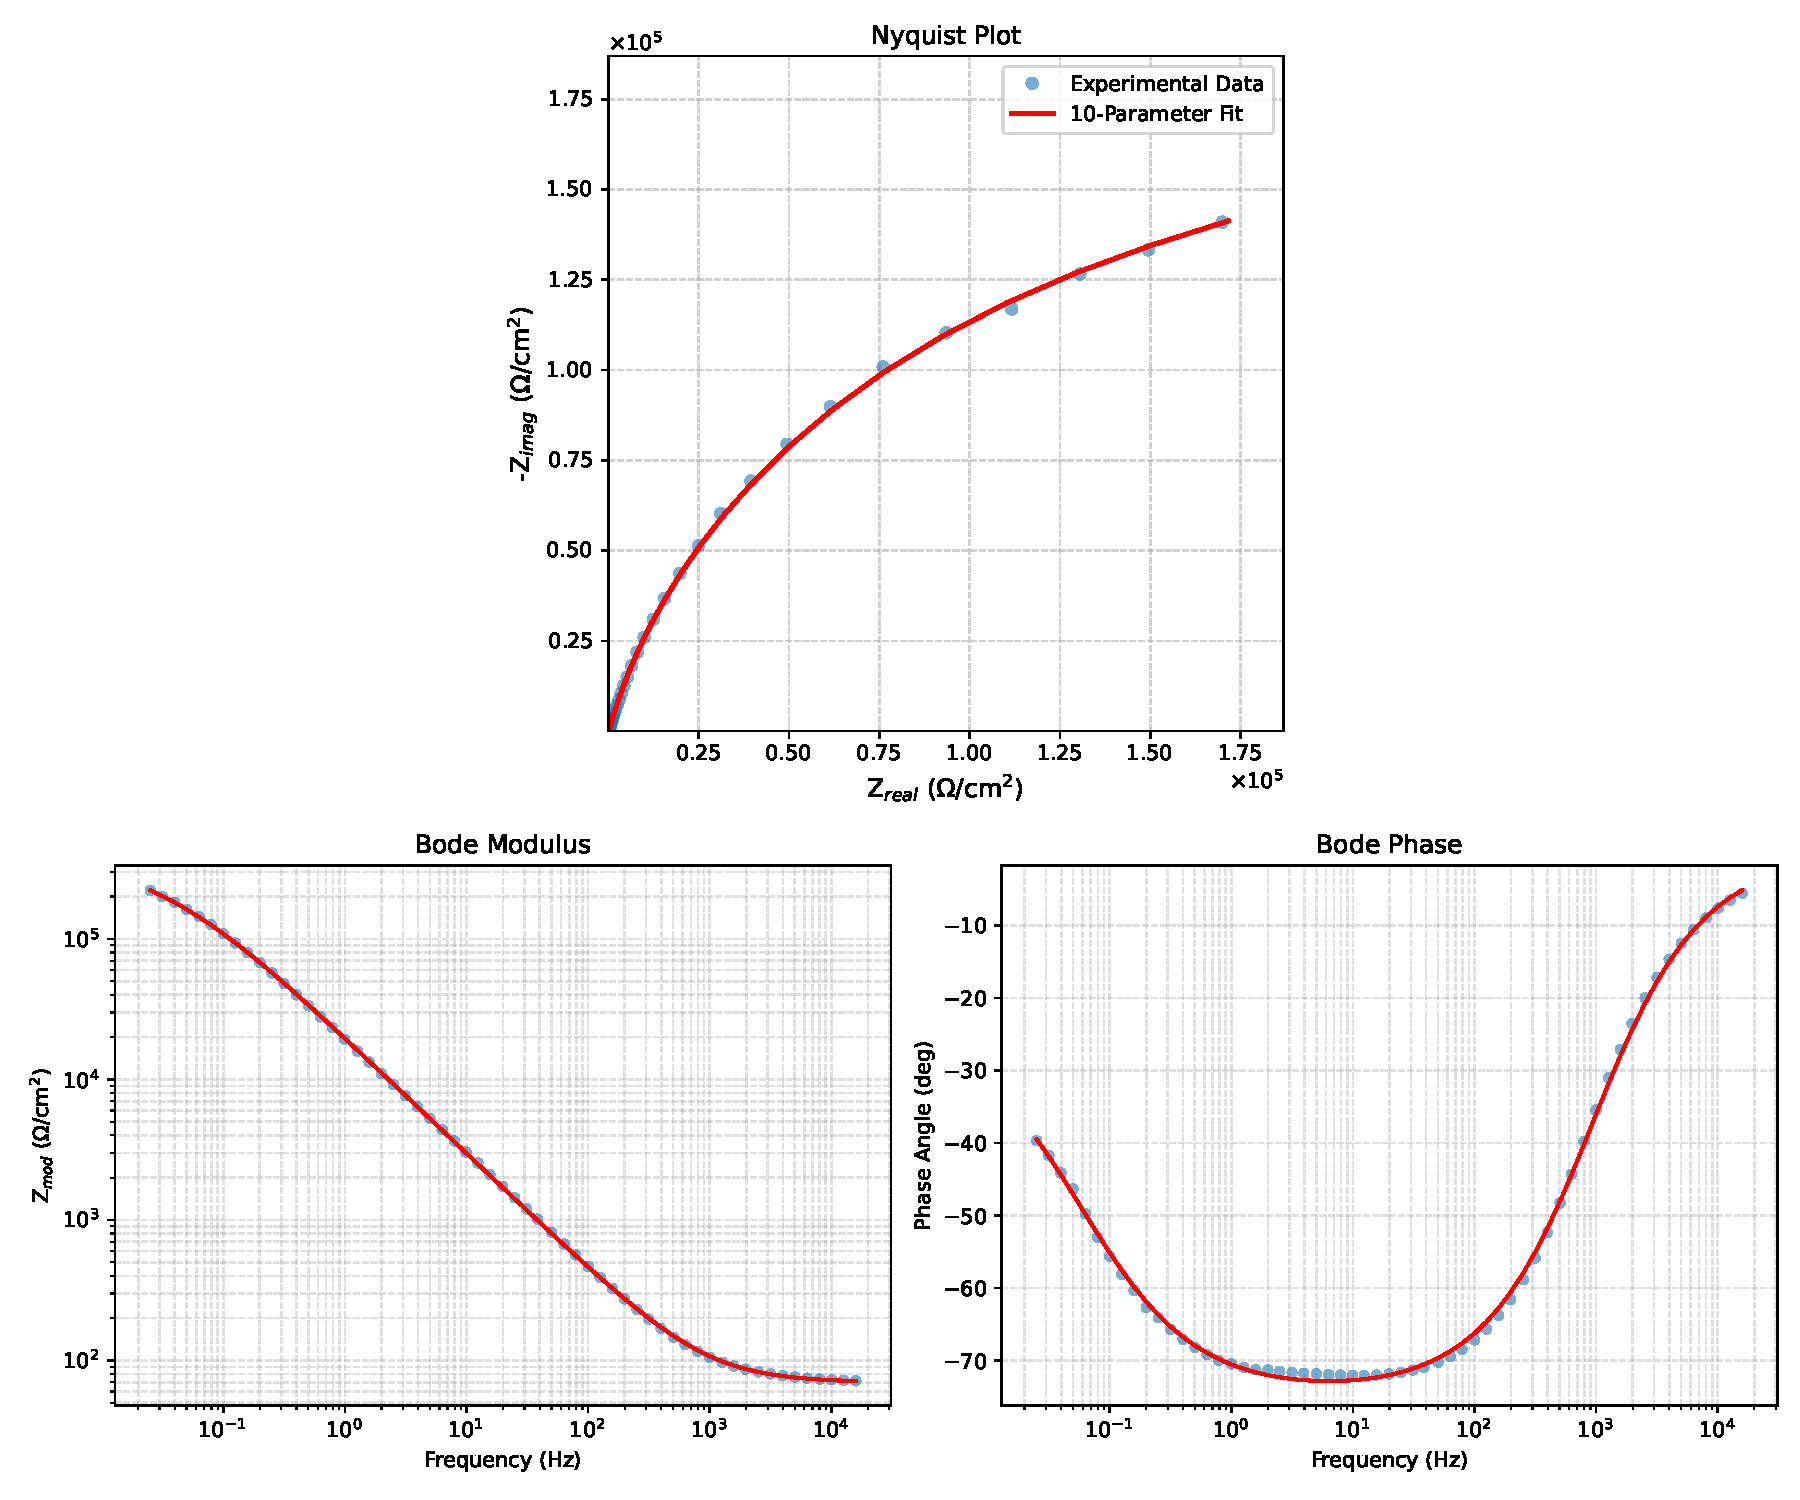
\includegraphics[width=0.7\textwidth]{plots_Cauvel_4_NaVO3_168H_2RC.pdf}
    \captionof{figure}{EIS Fit Results for Cauvel\_4\_NaVO3\_168H}
\end{center}


\end{document}
